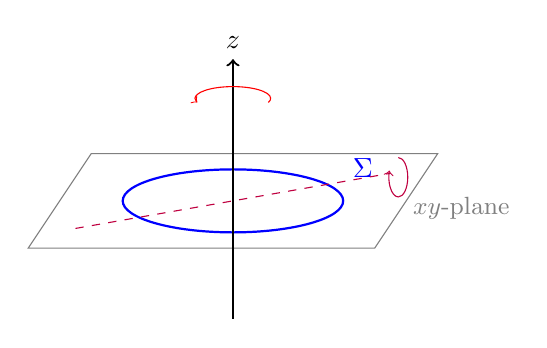
\begin{tikzpicture}[scale=1]
  % xy-plane as a parallelogram
  \draw[gray] (-2.6,-0.6) -- (1.8,-0.6) -- (2.6,0.6) -- (-1.8,0.6) -- cycle;
  \node[gray, font=\small] at (2.9,-0.1) {$xy$-plane};
  % circle Sigma (ellipse in perspective)
  \draw[thick, blue] (0,0) ellipse (1.4 and 0.4);
  \node[blue] at (1.65,0.42) {$\Sigma$};
  % z-axis
  \draw[->, thick] (0,-1.5) -- (0,1.8) node[above] {$z$};
  % rotation arrow about z
  \draw[->, red] (0.45,1.25) arc[start angle=-20, end angle=200, x radius=0.48, y radius=0.15];
  % a line in the xy-plane for the 180-degree flip
  \draw[dashed, purple] (-2.0,-0.35) -- (2.0,0.35);
  \draw[->, purple] (2.1,0.55) arc[start angle=90, end angle=-200, x radius=0.12, y radius=0.25];
\end{tikzpicture}
